\subsubsection{\stid{2.06} Exa-PAPI}\label{subsubsect:exapapi}

\paragraph{Overview} 

%Understanding the performance characteristics of exascale applications is 
%necessary in order to identify and address the barriers to achieving performance 
%goals. This becomes more difficult as the architectures become more complex. 
%The Performance Application Programming Interface (PAPI) provides both library 
%and application developers with generic and portable access to low-level 
%performance counters found across the exascale machine, enabling users to see
%the relationships between software performance and hardware events. 
%These relationships provide a critical step toward improving performance.

The Exa-PAPI 
project is developing a new C++ Performance API (PAPI++) software package 
from the ground up that offers a standard interface and methodology for using
low-level performance counters in CPUs, GPUs, on/off-chip memory, interconnects, 
and the I/O system, including energy/power management. 
PAPI++ is building upon classic-PAPI functionality and strengthening its path to
exascale with a more efficient and flexible software design, one that takes 
advantage of C++'s object-oriented nature but preserves the low-overhead 
monitoring of performance counters and adds a vast testing suite.

In addition to providing hardware counter-based information, a standardizing layer 
for monitoring software-defined events (SDE) is being incorporated that exposes 
the internal behavior of runtime systems and libraries, such as communication and 
math libraries, to the applications. As a result, the notion of performance events is 
broadened from strictly hardware-related events to include software-based 
information. Enabling monitoring of both hardware and software events provides 
more flexibility to developers when capturing performance information.


\paragraph{Key Challenges}

Widely deployed and widely used, PAPI has established itself as fundamental
software infrastructure in every application domain where improving performance
can be mission critical. 
However, processor and system designs have been experiencing radical changes.
Systems now combine multi-core CPUs and accelerators, shared and
distributed memory, PCI-express and other interconnects, and
power efficiency is emerging as a primary design constraint.
These changes pose new challenges and bring new
opportunities to PAPI. At the same time, the ever-increasing importance of
communication and synchronization costs in parallel applications, as well as the
emergence of task-based programming paradigms, pose
challenges to the development of performance-critical applications and create a
need for standardizing performance events that originate from various ECP
software layers.


\paragraph{Solution Strategy}

The Exa-PAPI team is preparing PAPI support to stand up to 
the challenges posed by exascale systems by 
\begin{enumerate}
\item widening its applicability and providing robust support for exascale 
hardware resources;
\item supporting finer-grain measurement and control of power, thus offering 
software developers a basic building block for dynamic application optimization 
under power constraints; 
\item extending PAPI to support software-defined events; and 
\item applying semantic analysis to hardware counters so that the application 
developer can better make sense of the ever-growing list of raw hardware 
performance events that can be measured during execution. 
\end{enumerate}

%The Exa-PAPI effort delivers new PAPI components to handle the wide range of
%new hardware and software events for the extreme scale platforms that will form
%the basis of exascale computing. To achieve this, Exa-PAPI implements a variety
%of monitoring and sampling capabilities for the different technologies, which
%are exported to the ECP application community. 
%%
%Exa-PAPI also provides finer-grain measurement and control of power, thus
%offering software developers a basic building block for dynamic application
%optimization under power constraint. Other hardware efforts in Exa-PAPI are the
%development of components for monitoring network interconnect events, as well as
%components targeted at the deep and heterogeneous memory hierarchies that we
%are already seeing in new architectures.

In summary, the team will be channeling the monitoring capabilities of hardware 
counters, power usage, software-defined events into a robust PAPI++ software 
package. PAPI++ is meant to be PAPI's replacement---with a more flexible and 
sustainable software design.


\paragraph{Recent Progress}

The Exa-PAPI team shipped the PAPI 6.0.0 release on March 4, 2020. This release 
includes a new API for Software Defined Events (SDEs), a major revision of the 
high-level API, and several new components, including ROCm and ROCm\_{SMI} for AMD GPUs, 
powercap\_{ppc} and sensors\_{ppc} for IBM Power9 and later, the SDE component to expose 
software-defined events through the standard PAPI interface, and the IO component that 
exposes I/O statistics exported by the Linux kernel. 

\vspace{10pt}
Furthermore, PAPI 6.0.0 ships CAT, a new Counter Analysis Toolkit that assists with native 
performance counter disambiguation through micro-benchmarks. 
Performance in different CPU architectures can be monitored by reading the occurrences 
of various hardware events. However, from architecture to architecture, it is not clear which 
native hardware events are indexed by which event names, making it difficult for the 
performance analyst to understand how to measure specific events.
To alleviate this difficulty, CAT aims to measure the occurrences of events through a series 
of benchmarks, classify particular events of interest via data analysis of the patterns of 
event occurrences, and allow its users to discover the high-level meaning of native events.
%
The examples in Figure~\ref{fig:cat_flops} show the results from the CAT floating-point tests used to 
verify single- and double-precision FLOP counters on three different CPU architectures 
(Intel Broadwell, Intel Skylake, IBM POWER9 CPU). Our paper~\cite{toolsWS-2020-09} discussed 
how to monitor bandwidth and arithmetic intensity with PAPI and CAT.
%
\begin{figure}[!h]
\begin{center}
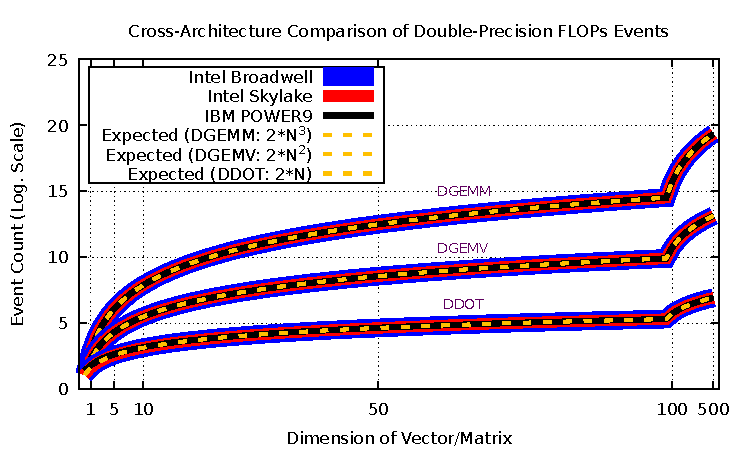
\includegraphics[width=0.7\linewidth]{projects/2.3.2-Tools/2.3.2.06-EXA-PAPI/cat-DP-flops-arch-comparison-1.pdf}
\caption{FLOPs validation on Broadwell, Skylake, and POWER9.}
\label{fig:cat_flops}
\end{center}
\end{figure}
%\vspace{-8pt}



%\vspace{10pt}
For the refactoring PAPI to PAPI++ effort, the Exa-PAPI team circulated a survey to the ECP 
applications AD and ST teams to assess their needs and requirements 
for hardware and software performance counter functionality. A white paper~\cite{PWN-2020-01} has been released, 
describing our survey findings and articulating research priorities for the development of the new 
PAPI++ software package.
In July 2020, a second white paper~\cite{PWN-2020-07} has been released, describing our roadmap for 
refactoring PAPI to PAPI++. The objective of these documents is to describe the current design of the
classic PAPI framework in conjunction with its limitations and sustainability challenges, as well as identify 
and articulate opportunities and possible implementations and C++ features for PAPI++ to provide support 
for the simultaneous measurement of data from multiple counter domains.



\paragraph{Next Steps}

Our next efforts will focus on:
\begin{enumerate}
\item \textbf{Production-ready CMake build system for PAPI++:} 
		Implementation of a production-ready CMake build system for PAPI++ .  
		We will build on the prototype CMake implementation from classic PAPI (produced in STTO09-103), 
		and use the "PAPI Red Team" input and feedback for implementing a CMake build system for the new 
		PAPI++ framework and its component.
%
\item \textbf{Transition from PAPI's C framework to the new PAPI++ framework implemented in C++}: 
		Implementation of the modular structure of the new PAPI++ framework that includes a new 
		C++ API in addition to the traditional C and Fortran APIs to preserve backward-compatibility. 
		Focus will be on the implementation of the PAPI++ core and modular framework that is 
		architecture-neutral. We will build on the design and prototype implementation from STTO09-105. 
		A beta release for early users will be planned as completion criteria. It will allow us to follow an 
		iterative and incremental software development process early in the design cycle before 
		adding all of the 30+ PAPI components to the new PAPI++ framework.
%
\item \textbf{Development of a C++ API for PAPI's stand-alone SDE library}:
		In addition to the already implemented and released C and FORTRAN APIs for the PAPI 
		software-defined event (SDE) functionality (release with STTO09-104), we will develop a 
		C++ API for the stand-alone SDE library while maintaining its traditional APIs. The goal is 
		to achieve consistency by providing all three APIs (C++ , C, FORTRAN) across all PAPI++ 
		modules. This effort involves transitioning PAPI SDE to the new PAPI++ package.
%
%\item \textbf{Transition PAPI's non-CPU components to the new PAPI++ software}:
%		Finalize the modular structure of the PAPI++ framework and transition the 
%		architecture-dependent (CPU, GPU, network, power, etc) PAPI components to the new 
%		PAPI++ implementation. New modules, enabling performance counter monitoring for novel 
%		and advanced ECP hardware and software technologies, will be developed in parallel and 
%		added incrementally with regular testing as new components are developed. This incremental 
%		process exposes performance problems or other issues early and allows them to be addressed 
%		in isolation. This effort involves a managed transition away from our legacy PAPI software while 
%		continuing to add support for new ECP hardware.
\end{enumerate}
